\subsection{The rate of inappropriate therapy}
\label{sec:rate inapp}
%\todo[inline]{justify episode-level rates and not patient-level}
The first objective of the MBCT is to estimate the rate of inappropriate detection $\bar{t}$ for each of the two algorithms for all arrhythmias combined, i.e., for the entire synthetic cohort.
The rate of inappropriate therapy is defined as
\[\bar{t} = \frac{\text{Number of inappropriately applied therapies}}{\text{Number of applied therapies}}\]
From this we can confirm or invalidate the assumption that Rhythm ID outperforms PRL+W.
We generated a synthetic cohort of 11,400 heart instances, equally distributed among the 19 arrhythmias.
The number of instances was obtained from a Monte Carlo calculation.% whose details follow the presentation of the results.

\textbf{Conclusion 1: PRL+W delivers less inappropriate therapy.}
The obtained rates of inappropriate detection were 6.65\% for Boston Scientific and 2.91\% for Medtronic (P < 0.0001), assuming an equal number of patients from each arrhythmia in the synthetic cohort.
The corresponding relative improvement \emph{of Medtronic over Boston Scientific} is 56\%.
In other words, the MBCT reveals that the PRL+W algorithm from Medtronic actually differentiates between VT and \ac{SVT} better than Rhythm ID from Boston Scientific.
Our findings are consistent with the observations of the RIGHT trial itself~\cite{GoldABBTB11_RIGHTresults}.

\textbf{Conclusion 2: result holds across population characteristics.}
The above rates were obtained under the assumption that each arrhythmia is equally represented in the cohort.
A significant feature of MBCT is that it allows us to study the endpoint of interest (here, rate of inappropriate detection) on a variety of populations, which have the various arrhythmias in different proportions.
This may not be feasible in a real clinical trial, which has to contend with the population present at the clinical centers where the trial is conducted.
We may then ask: does PRL+W maintain a lower rate of inappropriate detection across different populations?
To answer this question, we varied the distribution of the arrhythmias in the synthetic cohort, and re-computed the cohort-wide rates of inappropriate therapy.
Fig. \ref{fig:popvar8} shows the results for 10 random variations of the arrhythmia distribution.
It can be seen that indeed, PRL+W maintains a better rate of arrhythmia discrimination (and by inference, less inappropriate therapy) across the board.
%Thus the results are robust to the characteristics of the population under study.
%\mynote{SD}{Delete last sentence}

\begin{figure*}[t]
	\vspace{-10pt}
\centering
\vspace{-10pt}
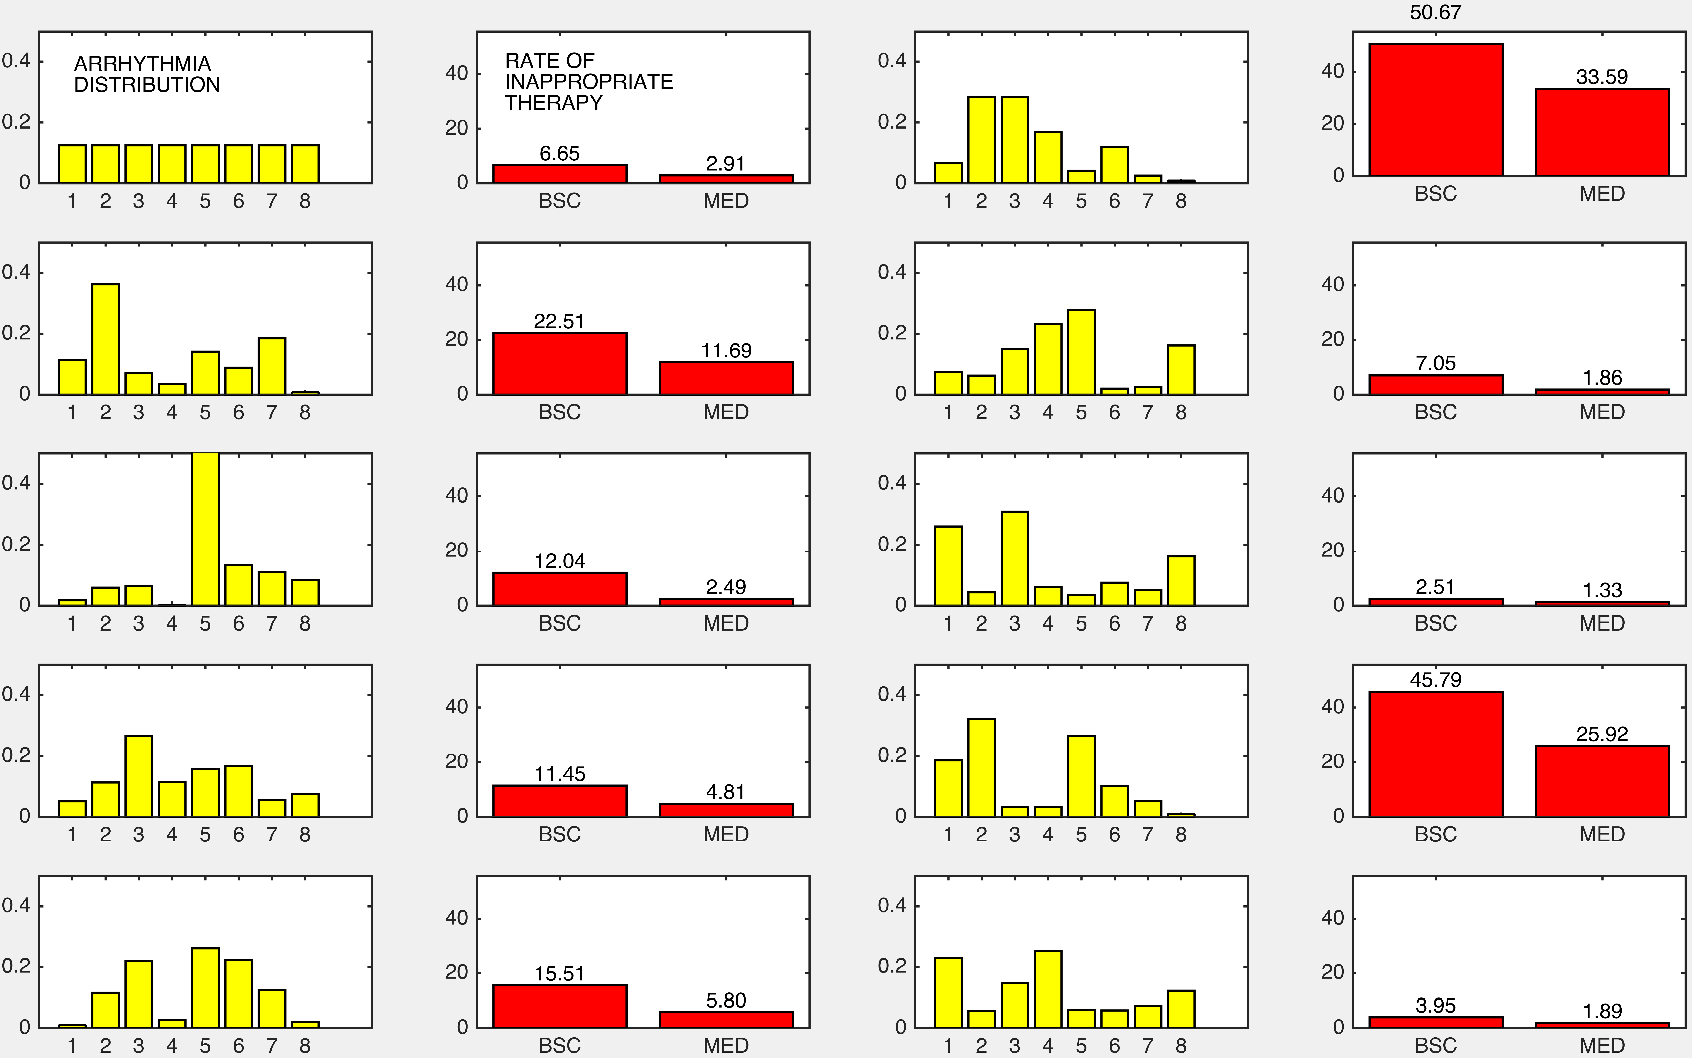
\includegraphics[scale=0.4]{figures/popvar9}
\caption{\small Rate of inappropriate detection ($2^{nd}$ and $4^{th}$ columns) for different arrhythmia distributions ($1^{st}$ and $3^d$ columns). The arrhythmias are (left to right on the x axis): Atrial fibrillation, Atrial flutter, Premature Ventricular Complexes, Nonsustained Ventricular Fibrillation, Supraventricular Tachycardia, Sinus Brady-Tachy, Ventricular Fibrillation, Ventricular Tachycardia \cite{josephson}. The top left distribution is uniform, and the bottom right distribution is that of the baseline characterization in RIGHT \cite{GoldABBTB11_RIGHTresults}.}
\label{fig:popvar8}
\end{figure*}

This illustrates very well the benefit that an \ac{MBCT} can bring to the planning of an \ac{RCT}: the fact that Rhythm ID could not be shown to be better than PRL+W %(let alone 25\% better as was hypothesized by the investigators) 
can cause the investigators to re-consider their assumptions and the feasibility of the trial.
In this case, the \ac{MBCT} casts doubt on the assumed \emph{direction} of the effect, i.e. whether intervention is better than control, or the other way around.
This early check can mean the difference between an expensive trial that fails at showing the desired effect, and a trial that is appropriately sized to demonstrate the desired effect size.

%While we will not know the true distribution of the arrhythmias in the \ac{RCT} until its completion, 
Thus, while an MBCT does not replace or mimic the RCT since we can not capture patient-level outcomes of the therapy, it can provide  but \emph{early insight} at a small fraction of the RCT cost and duration and without the ethical issues.	 

%\textbf{Sample size calculation for MBCT}.
%The rate is naturally computed as the mean of a random variable.
%Namely, it is the mean of the variable $t$ which equals 1 if the episode is a VT/VF for which therapy was applied, and 0 if it's a VT/VF for which therapy was withheld.
%To get reliable estimates for this rate, we use a standard Monte-Carlo calculation under the assumption that the estimate of the mean is normally distributed around the true mean. 
%This is justified by the central limit theorem and the fact that we can generate a very large number of hearts for each rhythm.
%By choosing a confidence interval width of 0.001 around the mean, we obtain a sample size of 9,604 hearts.
%In our experiments we used 11,400 to decrease the empirical variance of the estimate.
%The 95\% confidence interval around the mean estimate is given by $CI = \hat{t} \pm z_{95}\frac{S_t}{\sqrt{n}}$, 
%where $\hat{t}$ is the mean estimate, $z_c$ is the $c\%$ confidence level (so $z_{95}=1.96$), 
%$S_t$ is the empirical variance, 
%and $n$ is the number of Monte Carlo simulations, i.e., the number of heart instances we will generate and simulate for a given rhythm.
%The larger the number of simulations $n$, the tighter the confidence interval around the estimate.
%The rates we estimate fall in the range $[0,1]$ and are significant to the second decimal digit.
%Because we are considering all arrhythmias combined, we assume a conservative empirical variance $S_x$ to be 0.05, (validated experimentally) and set the desired confidence interval half-width to 0.001:
%\[\1.96\frac{0.05}{\sqrt{n}} = 0.001\]
%This yields $n = 9604$.
%In the experiments we use $n=11400$ to help guarantee the assumed empirical variance.
%The obtained empirical variance is invariably much smaller than 0.05.

%The obtained results for sensitivity and inappropriate therapy rate are shown 
%\begin{table}[b]
%	\smallcaption{Sensitivity and inappropriate therapy rate.}
%	\begin{tabular}{|p{1.9cm}|c|p{2.5cm}|}
%		\hline             & \textbf{Boston Sci.}(\%)   & \textbf{Medtronic} (\%)\\
%		\hline Sensitivity &  100                   &  100  \\ 
%		\hline Inappropriate therapy rate &  6.65                   &  2.91 \\ 
%		\hline 
%	\end{tabular}
%	\label{table:total nbs}
%\end{table} 

%We may also define a hypothesis test, which we illustrate for the rate of inappropriate therapy.
%The null hypothesis $H_{0,t}$ is that the rates for $\bar{t}$ are equal for Medtronic and Boston Scientific devices.
%\[H_{0,t}: \bar{t}_{MED} = \bar{t}_{BSC}  \]
%The alternative hypotheses are that the rates are not equal.
%In all that follows, `effect size' refers to the relative difference between the two rates.
%
%We assume an effect size of 27\%: this is based on the \emph{episode-level} inappropriate therapy rates reported in RIGHT (Table 2 of \cite{GoldABBTB11_RIGHTresults}).
%(Note that some of those reported results, however, were not statistically significant at the 5\% significance level).
%At the 5\% significance level and 90\% power, this yields a sample size of 11160.
%% with an assumed BSC rate of 0.08.
%We used 11400 instances in our MBCT.
%The results were inappropriate therapy rates $\bar{t}_{BSC}= 0.0291$ and $\bar{t}_{MED} = 0.0665$, with an effect size (relative to Medtronic's algorithm) of 56\% with $P << 10^{-3}$.
%Thus the null hypothesis of equality of inappropriate therapy rates can be rejected.

\subsection{Condition-level rates}
\label{sec:condition-level}
Having a heart model allows us to better estimate the \emph{sensitivity} and \emph{specificity} of the diagnostic algorithms' performance, something which is not possible in a clinical trial because the device only records a limited number of episodes.
These are defined as
\[ \text{Sensitivity} = \frac{\text{Number of correctly classified VTs}}{\text{Number of true VTs}}\]
\[ \text{Specificity} = \frac{\text{Number of correctly classified SVTs}}{\text{Number of true SVTs}}\]
In words, the sensitivity measures how well the device recognizes VTs.
Specificity measures how well the device discriminates between VT and SVT.
An ideal device would have 100\% sensitivity and specificity.
Unfortunately, these are typically competing goals: the more sensitive the device, the more likely it will mis-diagnose some SVTs as VTs, so its specificity will drop.
%During a clinical trial, the implanted ICD is typically set to record only treated episodes, so it is not possible to obtain all episodes and measure specificity.
%Moreover, if a VT episode is non-sustained, it won't receive therapy and won't be recorded, so it's not possible to measure sensitivity.
%Even if the device were set to record all episodes whether treated or not, memory limitations mean that it won't record everything.

We calculated sensitivity and specificity in our MBCT, and report them in Table \ref{table:vtsvt} on a per-arrhythmia basis.
The conditions are drawn from RIGHT's baseline characterization \cite{GoldABBTB11_RIGHTresults}.
Specificity is reported for SVTs and sensitivity is reported for VTs.
It can be seen from these results that in our synthetic cohort, Atrial flutter and other Supraventricular tachycardias are the main source of inappropriate detection for Rhythm ID compared to PRL+W.
In the case of Atrial flutter, Rhythm ID categorizes it inappropriately as \ac{VT} for 41.7\% of the cases.

Condition-level analysis pinpoints the specific pathways of the discrimination algorithm which must be addressed to reduce the device's rate of inappropriate therapy. It is difficult to get such insight through an RCT as the patient population is fixed and the conditions are determined retroactively. Such analysis can be further used to investigate condition distributions across different patient population types (e.g. abnormal heart rhythms in children vs geographic region-specific or race-specific condition distributions).   

\begin{table}[t]
	\vspace{-10pt}
	\smallcaption{Specificity and sensitivity.}
\begin{tabular}{|p{2.8cm}|p{1.5cm}|p{1.5cm}|c|}
	\hline Arrhythmia & Boston Sci. ICD & Medtronic ICDs  & P value \\ 
	\hline &	\multicolumn{2}{|c|}{\textbf{Specificity} (\%)}& \\
	\hline Atrial Fibrillation & 99.8 & 99.6 & 0.3167 \\ 
	\hline \cellcolor{blue!25} Atrial flutter & 58.3 & 79.33 & <0.0001 \\ 
	\hline Premature ventricular complexes & 100 & 100 & 1 \\ 
	\hline Nonsustained ventricular tachycardia & 100 & 99.8 & 0.3171 \\ 
	\hline \cellcolor{blue!25} Other Supraventricular tachycardia & 96.3 & 99.7 & <0.0001 \\ 
	\hline Brady-Tachy & 100 & 98.83 & 0.0079 \\ 
		\hline
	\hline &	\multicolumn{2}{|c|}{\textbf{Sensitivity} (\%)} & \textbf{P value}\\
	\hline Ventricular fibrillation & 100 & 100 & 1 \\ 
	\hline Ventricular tachycardia & 100 & 100 & 1 \\ 
	\hline 
\end{tabular} 
\vspace{-10pt}
\label{table:vtsvt}
\end{table}